\section{Introduction}
In this appendix is presented the application developed to test the data synchronization capabilities of CPIM, while persisting data through the Datastore Kundera extension. 

\section{Hegira generator}
\label{sec:hegira-generator}
To be able to test the interaction between the CPIM library and the synchronization system, and to provide an example of usage of the extended CPIM library, we have developed \textit{Hegira generator}.

\noindent The application provides two behaviors through command line interface, a \texttt{clean} command to clean-up the remote Datastore instance by deleting all the entities of all Kinds, and a \texttt{generate} command, that takes as argument the number of entities, per table, to be generated and generates them.

\newparagraph Data generation is done upon a pre-defined entity model inside the application and described by the ER diagram of Figure \ref{fig:hegira-generator-er}.
Building an entity generator agnostic to the entities model was not our goal and it would have required a way to automatically build the dependency graph of the entities since entities related to other ones, should have a reference to the entity they depend on. Hence the application is aware of the entities dependencies and generates them accordingly.

\begin{figure}[tbh]
  \centering
  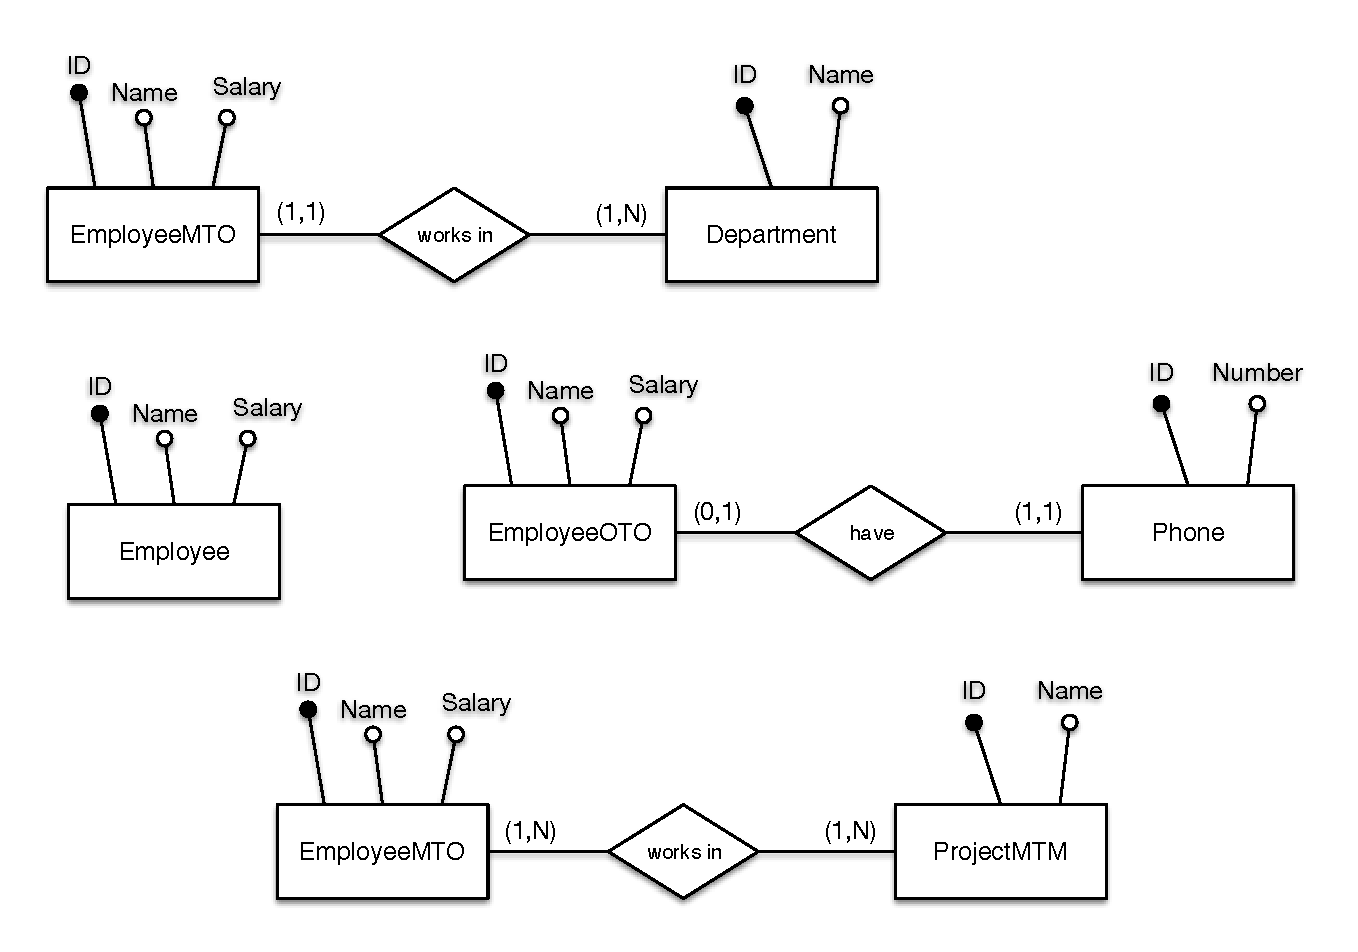
\includegraphics[width=10cm]{images/hegira_generator_er}
  \caption{ER diagram of Hegira-generator model}
  \label{fig:hegira-generator-er}
\end{figure} 

\noindent To be able to generate random entities, two methods are used:
\begin{itemize}
\item \texttt{persist(Class master)} that generates and persists entities without dependencies (such as \texttt{Employee} in the application model);
\item \texttt{persist(Class master, Class slave, DependencyType type)} that generates and persists the entities of the \textit{master} class and then uses randomly extracted entities among those just generated to fill the dependencies for the entities of the \textit{slave} class.
The \texttt{DependencyType} would be \texttt{SINGLE}, if the \textit{slave} class needs just one element to fill the dependency (which is the case of \textit{One to One} and \textit{Many to One} relationships), or \texttt{COLLECTION}, if the \textit{slave} class needs more than one element to fill the dependency (which is the case for \textit{Many to Many} relationships).
\end{itemize}

\noindent The actual entity generation is delegated to the entity itself through reflection since each entity of the model implements the \texttt{Randomizable} interface.
An example of entity genearion through this interface is shown in the snippet \ref{code:randomizable}.

\begin{lstlisting}[language=Java, caption=Entities generation, label=code:randomizable]
@Entity
public class EmployeeOTO implements Randomizable<EmployeeOTO, Phone> {
    ...
    @Override
    public EmployeeOTO randomize(Phone dependency) {
        setName(RandomUtils.randomString());
        setSalary(RandomUtils.randomLong());
        setPhone(dependency);
        return this;
    }
}
\end{lstlisting}
 
\subsection{Exploited CPIM features}
To perform the persist operation of the generated entities we used the \texttt{EntityManager} interface on which we called the \texttt{persist} method. This is completely JPA compliant and the user is not aware of what is done under the hood since communication with the synchronization system is handled automatically. An example is provided in the code \ref{code:example-persist}.

\begin{lstlisting}[language=Java, caption=Persisting entities in CPIM, label=code:example-persist]
CloudEntityManager em = MF.getFactory().getEntityManager();
Department dep = new Department("Computer Science")
em.persist(dep)
\end{lstlisting}

\noindent The persist operation through \texttt{CloudEntityManager} contacts the synchronization system to get the assigned sequence numbers for the specific tables and assigns the first of them to the entity before delegating to Kundera the persist operation.

\newparagraph The application makes use of the possibility of modifying at run-time the size range that is requested to the synchronization system. Hence before the persist operation, the size of the sequence number range is set to the double of the number of entities to be generated. This is done through a call to \texttt{SeqNumberProvider.getInstance().setOffset(tableName, offset)}, if the resulting range size is grater than the maximum size that can be requested, is limited to that value. 

\newparagraph The last feature that is exploited by the application is the backup of sequence numbers to file. The backup is configured in the \texttt{migration.xml} file, as described in the appendix \ref{app:migration}.
This permit to the application, when is restarted, to restore the sequence numbers without the need of contacting the synchronization system. Furthermore, to avoid execution of the persist operations on a table which entities generation was completed in a previous execution, a file with the list of the table completely generated is kept in the same folder specified for the sequence numbers backup files.
